\subsection{Отбор событий}

Отбор разбивается на несколько шагов. В начале пути отбираются полностью нейтральные события с тремя и более фотонами.
Причём от каждого фотона требуется, чтобы его энергия была больше \SI{30}{\MeVr} и полярный угол не тяготеет к вакуумной трубе.
Для таких событий вычисляется полная энергия $E_{\text{tot}}$ и импульс $P_{\text{tot}}$ системы частиц.
Характерное распределение представлено на рисунке~\ref{fig:EtvsPt5095}.
Сгущение событий около точки $P_{\text{tot}} = \SI{0}{\MeVr}$ и $E_{\text{tot}} = \sqrt{s}$ отвечаем искомым событием.
От этой группы тянется два хвоста под углами \ang{45} вверх и вниз.
Равное отколонение импульса $|P_{\text{tot}} - \SI{0}{\MeVr}|$ и энергии $|E_{\text{tot}} - \sqrt{s}|$
---
указание на то,
что данная девиация вызвана одной частицей.
Хвост уходящий вверх соответствует учёту излишней энергии в системе,
как правило такое соответствует тому,
что фотонным кластерам приписывается излишнее энерговыделение или имеется дополнительный кластер не возникший в следствие $e^+e^-$-аннигиляции,
к которой относится конкретное событие.
Хвост уходящий вниз, наоборот свидетельствует о недостатке энергии-импульса в системе.

\begin{figure}
	\centering
	\label{fig:EtvsPt5095}
	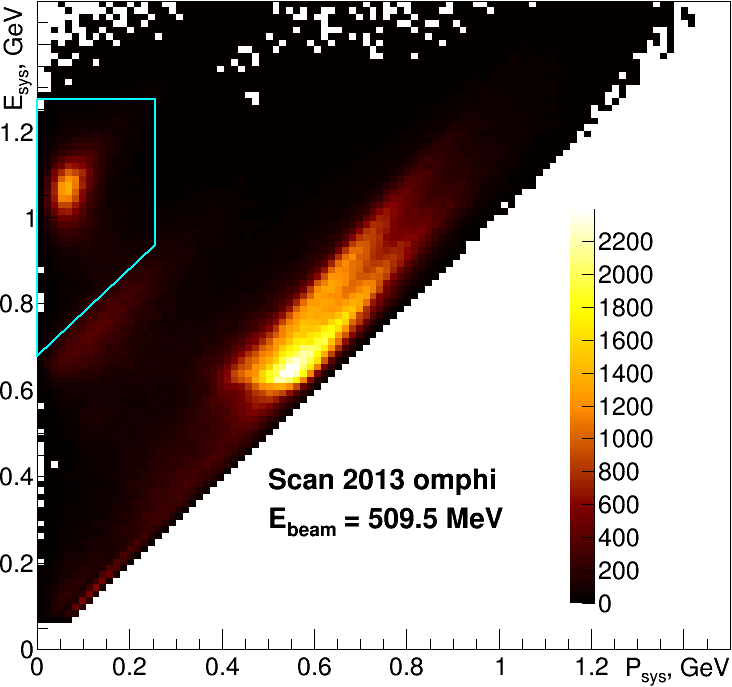
\includegraphics[width=.5\textwidth]{img/EtvsPt5095.png}
	\caption{Зависимость полной энергии события $E_{\text{tot}}$ от модуля полного импульса $P_{\text{tot}}$.
		Данные эксперимета, сезон 2013 $\omega \ \phi$, $E_{\text{beam}} = \SI{509.5}{\MeVr}$.
		Циановой линией обозначены условия отбора.}
\end{figure}

Теперь наступает шаг по отбору событий, в которых импульс системы близок к нулю,
а энергии к удвоенной энергии пучков.
Такой отбор направлен на те события,
где детектор зарегистрировал все частицы конечного состояния,
в то время как дополнительные кластеры в калориметре не дают значительного вклада.

На следующим шаге проводится кинематическая реконструкция событий.
В неё заложены законы сохранения энергии-импульса системы в целом и общая точка вылета фотонов.
Наличие промежуточных состояний $\pi^0$ или $\eta$ не требуется,
так как это оставляет крайне мало параметров последующей селекции сигнальных событий от фотона.
Если в событие присутствует более трёх фотонов,
то кинематическая реконструкция проводится для каждой возможной тройки и оставляется та,
что имеет наименьший $\chi^2$.
Подробнее о процедуре кинематической реконструкции изложено в разделе~\ref{sec:kf}.

Теперь, 
когда составлен набор трёхчастичных событий, 
отбрасываются все события, 
в которых не один из фотонов не полетел в центральную часть калориметра, 
а именно в систему \ce{LXe}. 
Такое условие предполагает наличие точки конверсии фотона,
определённой по полосковой электронике \ce{LXe} с хорошим координатным разрешением.

На этом отбор кандидатов закончен. 
В дальнейшем они разделяются на две большие пересекающиеся подгруппы: 
хотя бы один фотон попал в \ce{LXe} и все фотоны попали в центральную часть калориметра.
Попадание в центральную часть определяется по полярному углу фотона до кинематической реконструкции как $0.9 < \theta < \pi - 0.9$.



\subsubsection{Кинематическая реконструкция}
\label{sec:kf}

В ходе физической реконструкции событий закладывается гипотеза о знании точки вылета фотонов.
Предполагая угол влёта фотона в калориметр,
реконструируется его энергия по зарегистрированному энерговыделению.
Для нейтральных событий точка взаимодействия начальных лептонов не определена вдоль их движения и,
как следствие,
делается предположение о их вылете из центральной плоскости детектора $z = 0$.
Естественно,
это ухудшает разрешение параметров фотонов.
С целью преодоления такого недостатка проводится кинематическая реконструкция событий,
приводящая к улучшению ситуации,
что особенно ярко проявляется на распределениях инвариантных масс фотонов,
отвечающих мезонам.

Алгоритм кинематической реконструкции был разработан на основе работ \cite{Bukin2003-27, Bukin2005-51, Bukin2008-3}.
В них были описаны несколько подходов к составлению и минимизации функционалов.
Выбор остановился на составлении функционала со штрафными функциями,
сила которых регулируется весовыми коэффициентами
---
множителями Лагранжа.
Саму минимизацию было решено проводить численным методом.

В основу кинематической реконструкции заложены законы сохранения энергии-импульса системы в предположении общей точки вылета фотонов.

От энергии фотонов требуется, чтобы их сумма была равна сумме энергий пучков в системе центра масс. Последняя, в лучшем случае измерена с использованием обратного комптоновского рассеяния фотонов лазера на пучке. Следующая по приоритету информации энергии происходит из параметров частиц в различных физических процессах. Наихудший вариант --- уставная энергия ВЭПП-2000. Полный импульс системы полагается равными нулю. Эти два условия в купе говорят об отсутствие рассмотрения радиационного излучения как начальных, так и конечных частиц.
Логичным шагом развития кинематической реконструкции было бы добавления возможности уноса энергии и импульса вдоль оси пучков --- оси $z$.

Общая точка вылета определяется тремя координатами, две из которых фиксированы --- $x$ и $y$ берутся из дерева \textit{tr\_ph} для каждого захода (данный параметры усредняются по всем событиям в заходе с трековыми центральными вершинами в предположении стабильности орбиты пучков).
Разумеется, эти два параметра можно было бы отпустить, но их разрешение несравненно больше, чем у всех остальных, потому это можно отнести к категории мало-играющих факторов в ходе минимизации, разве что они увеличат затраченное время на процесс, и пренебречь ими. 
Третья координата $z$ точки взаимодействия свободна от каких-либо условий, другими словами, её разрешение бесконечно плохое и она не даёт вклада в $\chi^2$.

Когда говорят о координатах фотонов, подразумевается точка конверсии фотона в электрон-позитронную пару, 
являющуюся началом электромагнитного ливня в веществе детектора и не только. 
Определение этой точки конверсии сильно зависит от того, в каком месте она, конверсия, произошла.
Если рассматривать калориметры КМД-3, 
то при рождении ливня в \ce{LXe} в большинстве случаев срабатывает полосковая электроника, позволяя определить координаты с точностью \SIrange[range-phrase=--]{2}{4}{\mm} (?), 
либо по башням, если нет информации с полосок, но точность падает --- глубина равняется половине глубины башни а положение на цилиндрической поверхности средневзвешенному. 
В случае попадания фотона в \ce{BGO} калориметр $r$ и $\varphi$ координаты определяются по центру тяжести энерговыделения, 
а $z$ зависит от угла попадания фотона в калориметр в предположении вылета из центра детектора. 
Когда же фотон зарегистрирован только в \ce{CsI}, то $z$ и $\varphi$ определяются по центру тяжести, 
а $r$ устанавливается равной положению ближайшей к центру грани кристалла.

Координаты конверсии каждого фотона описываются в деревьях \textit{tr\_ph} параметрами $\rho$, $\theta$ и $\varphi$.
К двум последним прилагаются их ошибки $\sigma_\theta$ и $\sigma_\varphi$.
Так как $x_0$ и $y_0$ фиксированы,
то варьирование азимутального угла фотонов корректно.
Однако,
значение полярного угла определяется по точке вылета,
в том числе неопределённой точки $z_0$,
и точке конверсии фотона в калориметре.
Другими словами,
варьирование самого угла $\theta$ двигает две точки.
Поэтому необходимо их развязать для упрощение кинематической реконструкции.
Для цилиндрической части калориметра для варьирование выбирается координата $z$ точки конверсии,
связанная с полярным углом следующим образом:
\begin{equation}
    \theta_i
    =
    \arctg
    \frac{\rho_i}{z_i + \delta z_i + z_0} .
\end{equation}
Для торцевого калориметра варьирование идёт по координате $\rho$,
связь полярного угла с которой определяется как
\begin{equation}
    \theta_i
    =
    \arctg
    \frac{\rho_i + \delta \rho_i}{z_i + z_0} .
\end{equation}

Тем самым минимизация функционала производится варьированием $3 N + 1$ параметром



\begin{equation}
F = w_L L + w_W W + w_N \left( N_1 + N_2 + N_3 \right) + w_M M.
\end{equation}
$L$ отвечает за $\chi^{2}$
\begin{equation}
	L
	= 
	\sum_{i, \, \mu} 
	\frac{ \left( p^{i}_\mu -p^{fix,\,i}_\mu \right)^2 }{{\sigma^i_\mu}^2} , 
	\, \mu = E, \theta, \phi, \, i = \gamma_1, \gamma_2, \gamma_3.
\end{equation}
$W$ представляет закон сохранения энергии
\begin{equation}
	W = \left[ \sqrt{s} - E^{\gamma_1}- E^{\gamma_2}- E^{\gamma_3} \right]^2 ,
\end{equation}
$N_i$ --- закон сохранения импульса
\begin{equation}
	N_i = \left[ p_i^{\gamma_1} + p_i^{\gamma_2} + p_i^{\gamma_3} \right]^2, \, i=x,y,z ,
\end{equation}



\subsubsection{Определение числа сигнальных событий}

Определения числа сигнальных событий происходит по распределению инвариантных масс пар фотонов, иначе по массе отдачи одного из фотонов. Для каждой энергии и каждого  изучаемого процесса выбирается наиболее вероятная пара фотонов, в которую распался псевдоскалярный мезон. Стоит помнить, что фотоны упорядоченны по энергии $E_1 > E_2 > E_3$. Так в большой части диапазона доступных энергий для процесса $e^+ e^- \to \eta \gamma$ предпочтительна масса $m_{23}$, а для $\pi^0 \gamma$ --- $m_{23}$.

При построении таких распределений используется ряд дополнительных критериев на параметры частиц их системы в целом.
Минимальное число фотонов зарегистрированных в центральной части калориметра является одним из самых существенных таких отборов.
Для него используется два критерия,
либо хотя бы один фотон летит в цилиндрический калориметр,
либо все фотоны зарегистрированы в цилиндрической части.
Второй набор событий является подклассом первого.
Также второй набор аналогичен отборам проводимым при анализе на детекторе КМД-2,
что делает его более интересным для сравнения результатов.
Данный отбор даёт выбрать в пользу большей статистики или лучшего разрешения по инвариантной массе.

Вторым важным отбором является условие на минимальную энергию фотона,
как правило, она ставится равной \SI{50}{\MeVr}.
Данное число выбрано согласно моделированию и,
с одной стороны, подавляет фон в калориметре,
особенно в его торцевой части, с другой,
оказывает малое влияние на число сигнальных событий.
Таким образом возрастает отношение сигнал/фон.

Существует ещё условие на число зарегистрированных фотонов в событии.
В области $\phi$-мезона,
где сечение $e^+ e^- \to \eta \gamma$ достигает своего максимума,
это позволяет подавить вклад от канала распада $\eta \to \pi^+\pi^-\pi^0$,
ставя ограничение на число фотонов $n < 6$.

Непосредственно для определения числа сигнальных событий проводится подгонка распределения суммой сигнальной и фоновой функций.
Для описания фона используется полином.
Сигнал же описывается суммой нормальных распределений с общим нормировочным множителем.
Используемый алгоритм отбора событий также направлен на подавление фона,
что часто приводит к его малой статистике и трудности определения формы,
особенно под сигнальным пиком.
Для решения данной проблемы используется моделирование,
своё для каждой точки по энергии,
на которое опирается подгоночная функция --- так называемая одновременная подгонка (simultaneous fit).
В областях по энергии, где сечение мало,
и определение как числа событий сигнала,
так и фона затруднено привело к использованию небинированной подгонки,
которая позволяет в таких скользких ситуациях избежать проблем с выбором подходящего бинирования распределения.
Также для малой статистики вопрос, как правило,
идёт о определении верхнего предела, что, как временное решение,
приводит к определению асимметричных ошибок с помощью алгоритма Minos.